\apendice{Documentación de usuario}

\section{Introducción}

Este apéndice muestra los requisitos que debe cumplir el usuario para ejecutar la aplicación, así como la forma de instalarla y utilizarla.

\section{Requisitos de usuarios}

Como este proyecto consiste en una aplicación web, el usuario únicamente necesita poder ejecutar un navegador compatible con JavaScript, hojas de estilo CSS, Bootstrap, jQuery y D3. Algunos ejemplos son:
\begin{itemize}
    \item Google Chrome
    \item Mozilla Firefox
    \item Microsoft Edge
    \item Apple Safari
    \item Opera
\end{itemize}

\section{Instalación}

No es necesario realizar ninguna instalación para este proyecto, ya que consiste en una aplicación web.

\section{Manual del usuario}

En primer lugar, el usuario debe abrir la aplicación mediante la siguiente URL: \url{https://marcosgasolas.github.io/TFG_C4.5_simulator}.

Al cargar, se nos abrirá la página principal de la web. La figura \ref{Fig_E.1} muestra como se vé la página principal.

\begin{figure}[htbp]
     \centering
     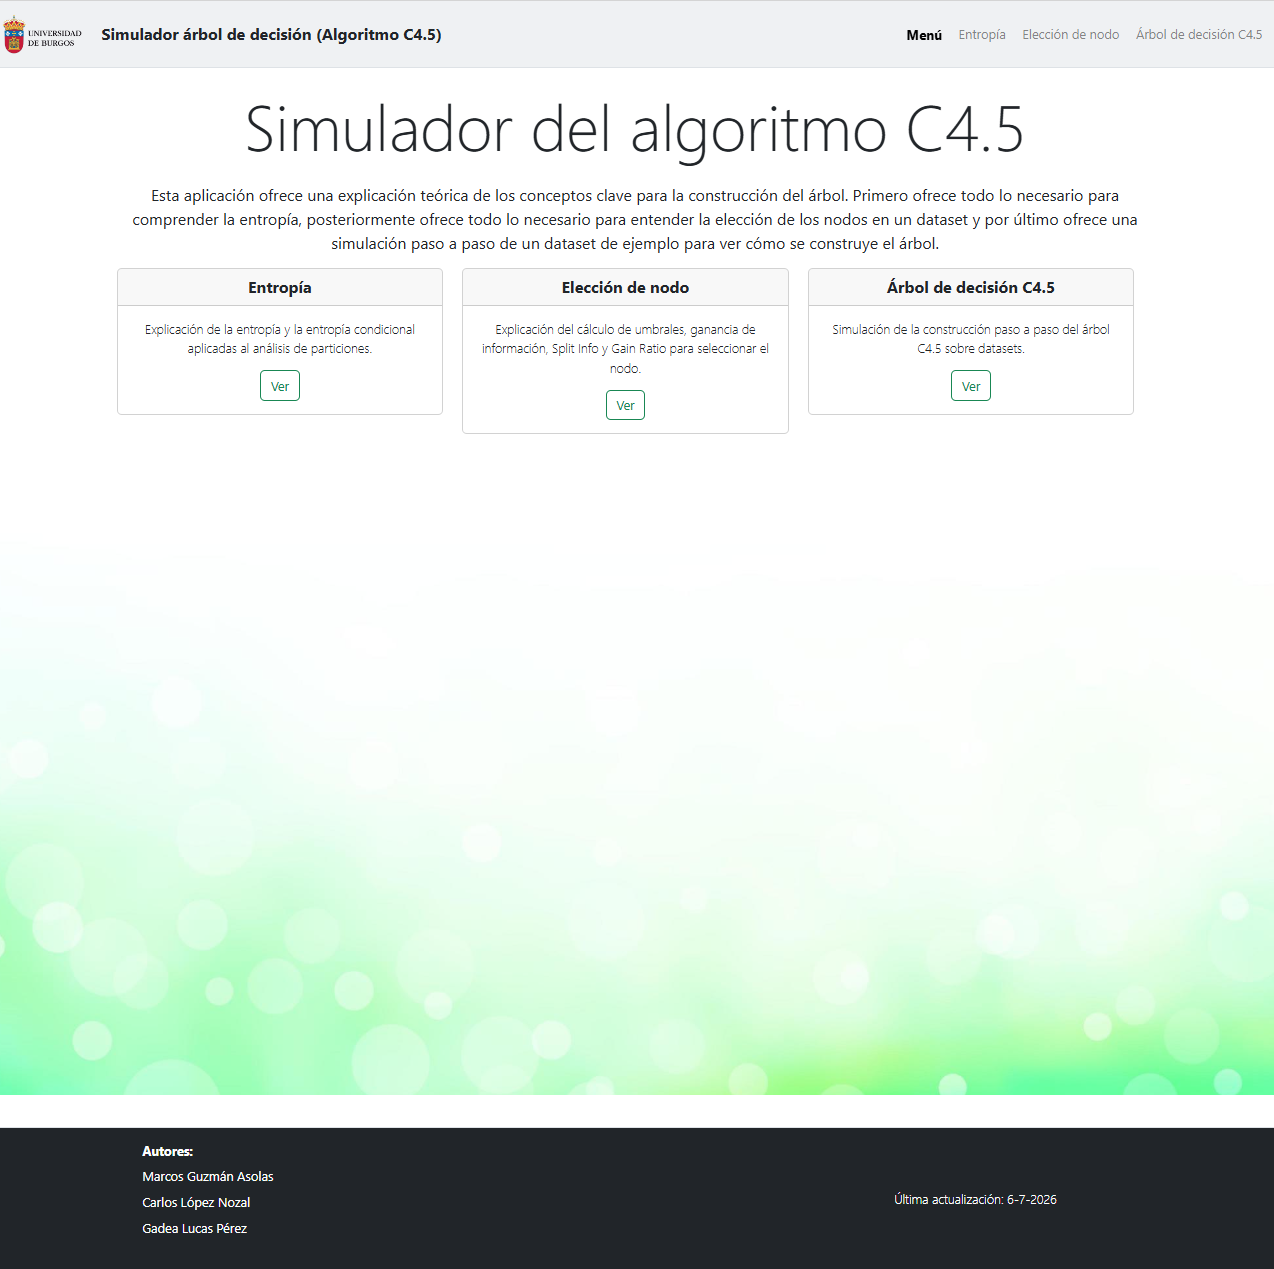
\includegraphics[width=1\textwidth]{img/Pagina_Principal.png}
     \caption{Visualización de la página principal de la web}
     \label{Fig_E.1}
 \end{figure}

 Además del título y de una breve introducción, se muestran tres tarjetas informativas, cada una correspondiente a una funcionalidad de la aplicación web, con la posibilidad de acceder a cualquiera de ellas: «Entropía», «Elección de nodo» y «Árbol de decisión C4.5».

\subsection{Entropía}
Si el usuario decide abrir la calculadora de entropía, se le muestra la página representada en la Figura~\ref{Fig_E.2}.

\begin{figure}[htbp]
     \centering
     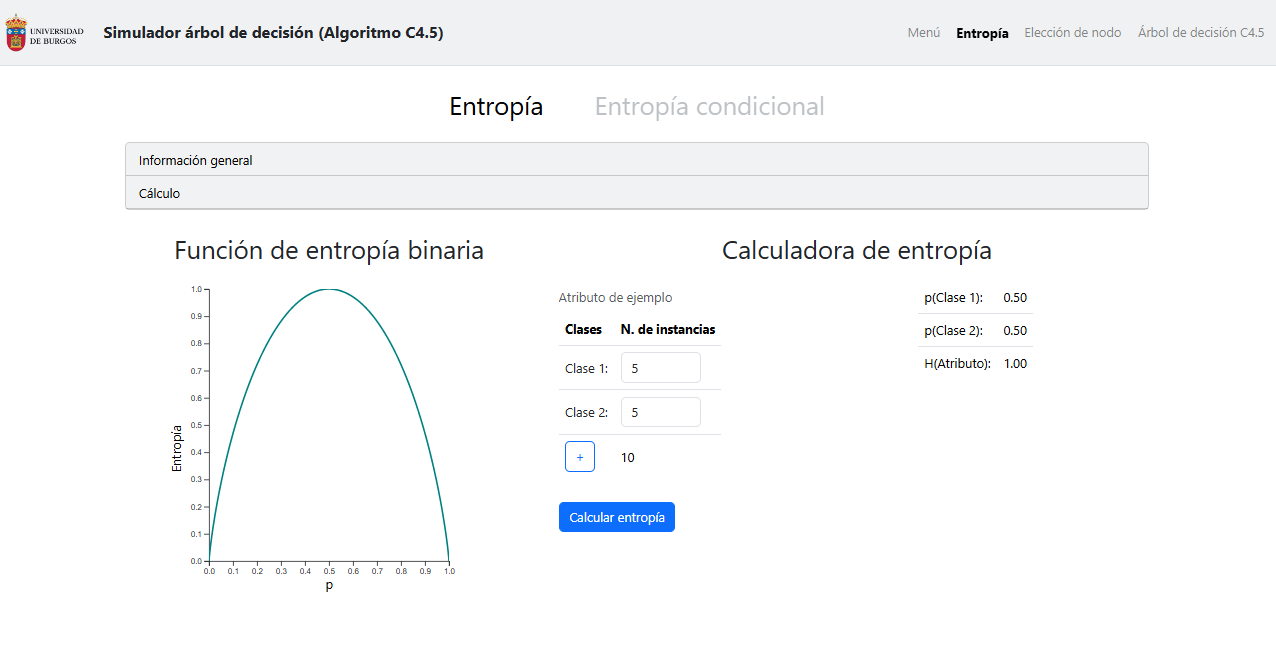
\includegraphics[width=1.2\textwidth]{img/Web_Entropia.png}
     \caption{Visualización de la página Entropía de la web}
     \label{Fig_E.2}
 \end{figure}

La página está formada por los siguientes componentes:
\begin{itemize}
    \item Tarjetas informativas en la parte superior.
    \begin{description}
        \item[Información general:] proporciona una breve introducción al concepto de entropía.
        \item[Cálculo:] muestra la fórmula de la entropía y explica cada una de sus partes.
    \end{description}
        \item Una gráfica situada a la izquierda que representa la función de entropía binaria.
        \item La calculadora de entropía situada a la derecha, formada por dos tablas.
    \begin{description}
        \item[Tabla izquierda:] representa un atributo de ejemplo cuyas instancias se distribuyen entre dos clases.
        \item[Tabla derecha:] muestra la proporción de cada clase en el conjunto de datos y la entropía del atributo.
    \end{description}
\end{itemize}

El usuario puede introducir cualquier valor entero positivo en los campos disponibles de la tabla izquierda y calcular la entropía para esos valores. Si se introducen valores no válidos, el usuario es informado mediante una alerta.

\subsection{Entropía Condicional}

La Figura \ref{Fig_E.3} muestra la página que se presenta al usuario al acceder a la calculadora de entropía condicional.

\begin{figure}[htbp]
     \centering
     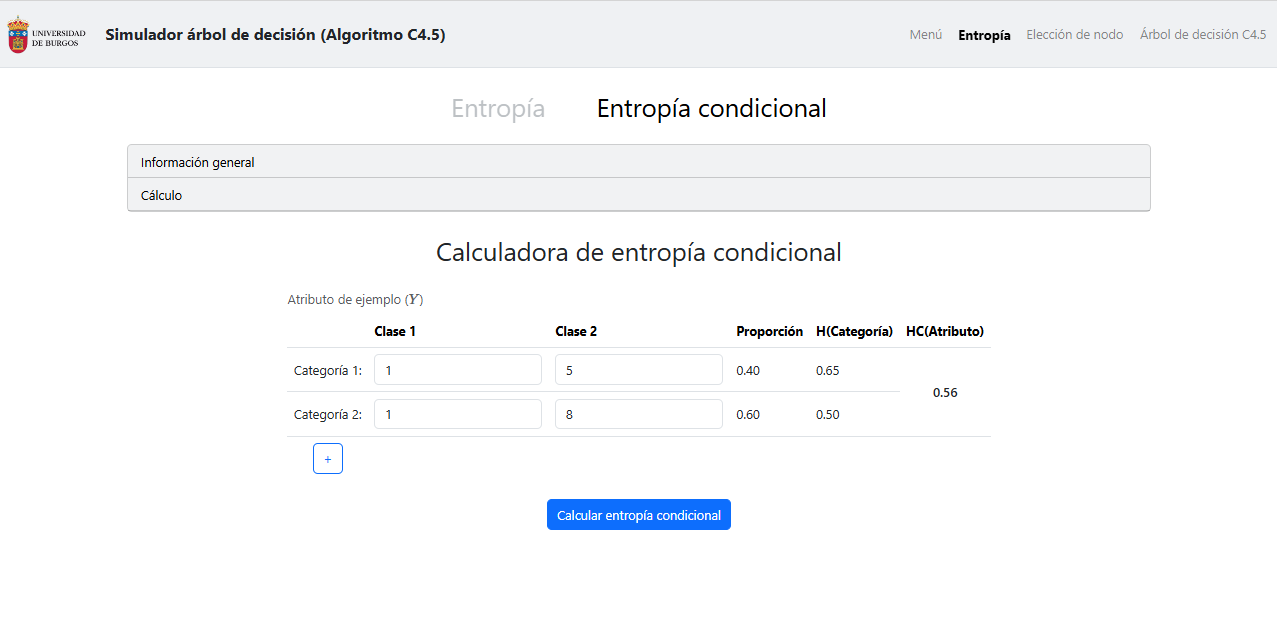
\includegraphics[width=1.2\textwidth]{img/Web_Entropia_Condicional.png}
     \caption{Visualización de la página Entropía Condicional de la web}
     \label{Fig_E.3}
 \end{figure}

La página contiene los siguientes elementos:
\begin{itemize}
    \item Tarjetas informativas en la parte superior.
    \begin{description}
        \item[Información general:] proporciona una breve introducción al concepto de entropía condicional.
        \item[Cálculo:] muestra las fórmulas utilizadas para calcular la entropía condicional y explica cada una de sus partes.
    \end{description}
    \item La calculadora de entropía condicional situada en la parte central.
\end{itemize}

De forma similar a la página de la calculadora de entropía, el usuario puede introducir cualquier valor entero positivo en los campos disponibles de la tabla y calcular la entropía condicional para dichos valores. Si se introducen valores no válidos, el usuario es informado mediante una alerta.

\subsection{Elección de nodo}

La pantalla se organiza mediante una barra superior de pasos, formada por las siguientes secciones:

\begin{itemize}
    \item \textbf{Umbral:} muestra cómo se calculan los posibles umbrales de división.
    \item \textbf{Ganancia de información:} permite analizar la reducción de entropía producida por cada umbral.
    \item \textbf{Split Info:} muestra el cálculo de la información de partición.
    \item \textbf{Gain Ratio:} calcula la métrica utilizada por C4.5 para comparar divisiones.
    \item \textbf{Nodo elegido:} presenta el umbral seleccionado como mejor nodo de decisión.
\end{itemize}

La figura \ref{Fig_E.4} muestra la página de cálculo de umbral en la sección de Elección de nodo de la web.

\begin{figure}[htbp]
     \centering
     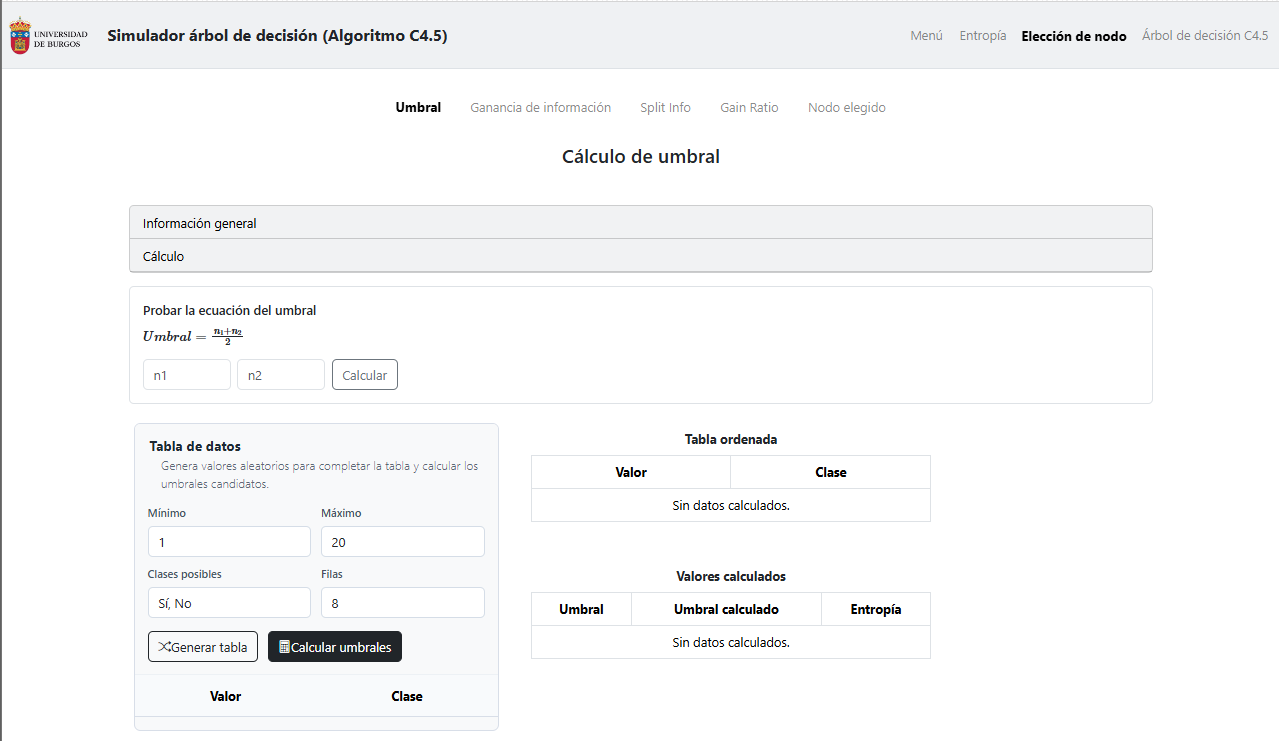
\includegraphics[width=1.2\textwidth]{img/Web_Eleccion_Nodo_Umbral.png}
     \caption{Visualización de la página Cálculo de umbral en la sección Elección de nodo de la web}
     \label{Fig_E.4}
 \end{figure}

La página contiene los siguientes elementos:
\begin{itemize}
    \item Tarjetas informativas en la parte superior.
    \begin{description}
        \item[Información general:] proporciona una breve introducción al concepto del umbral.
        \item[Cálculo:] muestra las fórmulas utilizadas para calcular el umbral.
        \item[Ecuación:] muestra la fórmula del umbral además de poder sustituir los valores para mostrar ejemplo de cálculo.
    \end{description}
    \item Tablas de datos para los cálculos del umbral.
    \begin{description}
        \item[Tabla de datos:] tabla de generación de datos para visualizar un ejemplo de cálculo del umbral
        \item[Tabla ordenada:] tabla ordenada con los datos generados de la tabla anterior.
        \item[Valores calculados:] tabla donde se muestran los valores calculados de la tabla de datos generada.
    \end{description}
\end{itemize}

La aplicación comprueba que estos valores sean válidos antes de crear la tabla. Por ejemplo, el mínimo no puede ser mayor que el máximo, el número de filas debe ser suficiente y las clases no pueden contener números. También se evita que los valores numéricos introducidos sean negativos. En la figura \ref{Fig_E.6} se muestra un ejemplo de la tabla de datos generados.

Una vez generada la tabla, el usuario puede pulsar el botón de cálculo correspondiente al paso actual. Este botón cambia de función según la sección en la que se encuentre:

\begin{itemize}
    \item en el paso de umbral, calcula los umbrales candidatos;
    \item en el paso de ganancia, calcula la ganancia de información;
    \item en el paso de \textit{Split Info}, calcula la información de partición;
    \item en el paso de \textit{Gain Ratio}, calcula la relación de ganancia;
    \item en el paso de nodo elegido, selecciona la mejor división.
\end{itemize}

Los resultados se muestran en una tabla situada junto a la tabla de datos, en la figura \ref{Fig_E.8} se muestra un ejemplo de esa tabla. En ella aparecen progresivamente las columnas necesarias para cada paso: valor, clase, umbral calculado, entropía, ganancia de información, \textit{Split Info} y \textit{Gain Ratio}. La tabla permite comparar los distintos umbrales candidatos y observar cómo evoluciona el proceso de selección.

La página también incluye elementos interactivos en las cabeceras y en algunas celdas de resultados. Al pulsar sobre determinados valores calculados, la aplicación puede completar automáticamente la calculadora manual correspondiente, permitiendo al usuario comprobar de dónde sale el resultado. Por ejemplo, se puede seleccionar un umbral calculado para ver los dos valores utilizados en su media, o pulsar sobre un valor de \textit{Gain Ratio} para cargar la ganancia y el \textit{Split Info} empleados en la división. En la figura \ref{Fig_E.7} se muestra un ejemplo de como dándole a una celda, nos muestra el calculo en la parte superior.

Cada paso dispone además de una calculadora manual específica. Estas calculadoras permiten introducir valores concretos y comprobar el resultado de forma independiente. Así, el usuario puede practicar el cálculo de umbrales, ganancia de información, \textit{Split Info} y \textit{Gain Ratio} sin depender únicamente de la tabla generada.

En el último paso, la aplicación muestra el nodo elegido. Este nodo corresponde al umbral con mejor \textit{Gain Ratio}. La visualización indica la condición de división y separa los datos en dos ramas: una para los valores menores o iguales al umbral y otra para los valores mayores. Si una rama contiene registros de una única clase, se muestra como resultado final; si contiene mezcla de clases, se indica que sería necesario seguir calculando nuevos nodos. En la figura \ref{Fig_E.9} se muestra un ejemplo de un nodo elegido.

La página incorpora también una leyenda desplegable cuando es necesario aclarar los colores o marcas usados en las tablas. Esta leyenda ayuda a interpretar qué filas intervienen en un cambio de clase, qué valores generan un umbral candidato y qué resultados han sido destacados. En la figura \ref{Fig_E.5} se muestra un ejemplo de una leyenda.

En conjunto, este módulo permite al usuario realizar las siguientes acciones:

\begin{itemize}
    \item navegar entre las fases del proceso de elección de nodo;
    \item consultar explicaciones teóricas y fórmulas de cada métrica;
    \item generar una tabla de datos aleatoria configurando rango, clases y número de filas;
    \item calcular umbrales candidatos para un atributo numérico;
    \item calcular la ganancia de información asociada a cada umbral;
    \item calcular el \textit{Split Info};
    \item calcular el \textit{Gain Ratio};
    \item identificar el mejor umbral como nodo elegido;
    \item utilizar calculadoras manuales para comprobar cálculos concretos;
    \item interactuar con celdas de resultados para cargar automáticamente valores en las calculadoras;
    \item interpretar los resultados mediante tablas, resaltados visuales y leyendas.
\end{itemize}

Este módulo actúa como paso previo a la simulación completa del árbol C4.5. Permite comprender con detalle cómo se toma una decisión individual antes de observar cómo el algoritmo repite este procedimiento de forma recursiva para construir el árbol completo.

\begin{figure}[htbp]
     \centering
     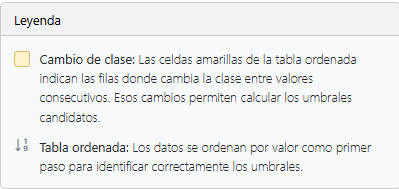
\includegraphics[width=0.75\textwidth]{img/Web_Leyenda.png}
     \caption{Visualización de la leyenda}
     \label{Fig_E.5}
 \end{figure}

 \begin{figure}[htbp]
     \centering
     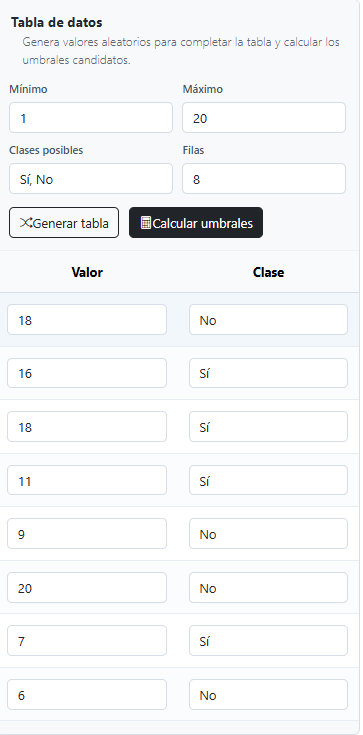
\includegraphics[width=0.5\textwidth]{img/Web_Tabla_Datos_Elección_Nodo.png}
     \caption{Visualización de la tabla de datos}
     \label{Fig_E.6}
 \end{figure}

 \begin{figure}[htbp]
     \centering
     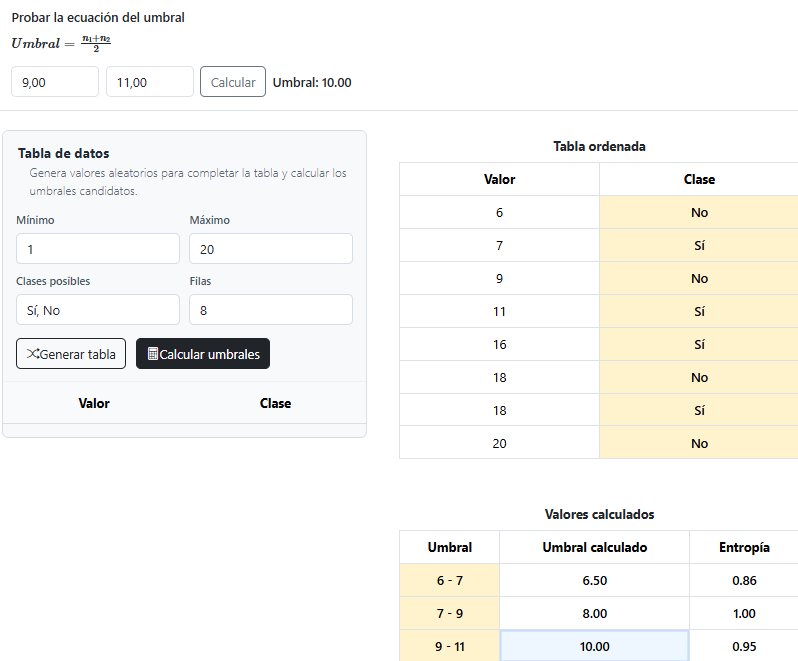
\includegraphics[width=1.2\textwidth]{img/Web_Navegacion_valores_calculados.png}
     \caption{Visualización de la navegación en la tabla de valores calculados}
     \label{Fig_E.7}
 \end{figure}

 \begin{figure}[htbp]
     \centering
     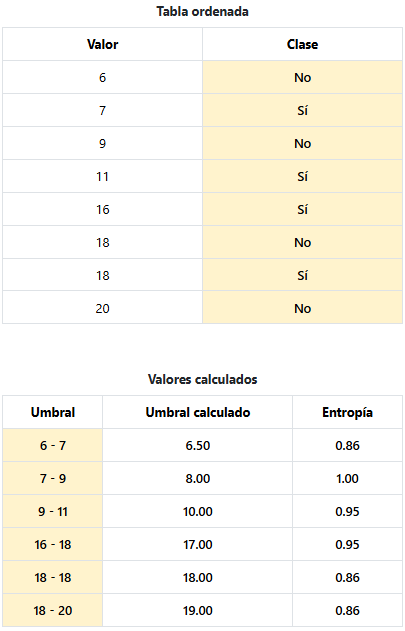
\includegraphics[width=0.75\textwidth]{img/Web_tablas_calculos_eleccion_nodo.png}
     \caption{Visualización de las tablas de valores calculados}
     \label{Fig_E.8}
 \end{figure}

 \begin{figure}[htbp]
     \centering
     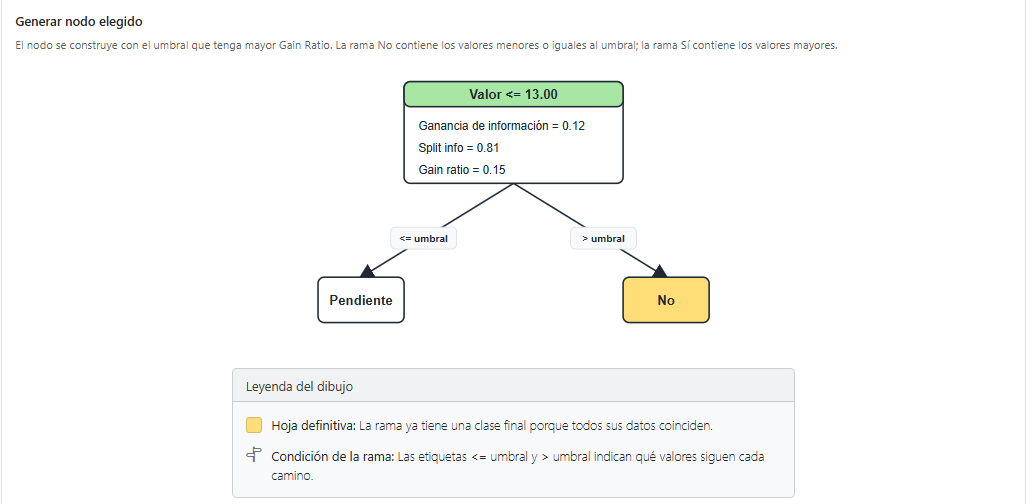
\includegraphics[width=1.2\textwidth]{img/Web_Ejemplo_Nodo_Elegido.png}
     \caption{Visualización de un ejemplo de un nodo en la parte de nodo elegido en la sección de Elección de nodos}
     \label{Fig_E.9}
 \end{figure}

 \subsection{Árbol de decisión C4.5}

El módulo de árbol de decisión C4.5 permite al usuario construir y visualizar un árbol de decisión completo a partir de un dataset. A diferencia de la sección de elección de nodo, donde se estudia una única decisión, esta página muestra cómo el algoritmo repite el proceso de selección de atributos y umbrales hasta generar la estructura completa del árbol.

La sección está dividida en dos apartados principales, accesibles desde la parte superior de la página:

\begin{itemize}
    \item \textbf{Simulación Árbol C4.5:} permite construir el árbol paso a paso.
    \item \textbf{Poda:} permite visualizar el proceso de simplificación del árbol generado.
\end{itemize}

La figura \ref{Fig_E.10} muestra la página principal de simulación del árbol C4.5.

\begin{figure}[htbp]
     \centering
     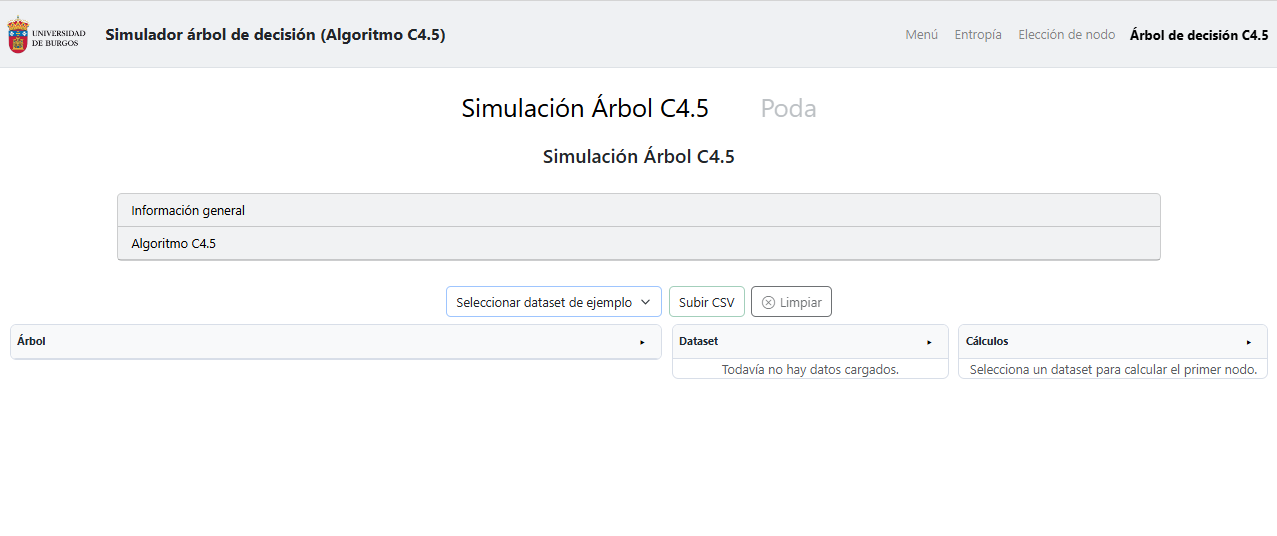
\includegraphics[width=1.2\textwidth]{img/Web_Arbol_C45.png}
     \caption{Visualización de la página de simulación del árbol C4.5}
     \label{Fig_E.10}
 \end{figure}

La página contiene, en primer lugar, tarjetas informativas desplegables. Estas tarjetas permiten al usuario consultar una explicación general del algoritmo y una descripción resumida de los pasos que sigue C4.5 para construir el árbol.

\begin{itemize}
    \item Tarjetas informativas en la parte superior.
    \begin{description}
        \item[Información general:] explica cómo C4.5 construye el árbol de forma recursiva, evaluando los atributos disponibles y seleccionando la mejor división.
        \item[Algoritmo C4.5:] muestra los pasos principales del algoritmo, incluyendo el tratamiento de atributos continuos, atributos categóricos, cálculo de métricas y condiciones de parada.
    \end{description}
\end{itemize}

Debajo de la información teórica se encuentran los controles de carga de datos. El usuario puede seleccionar uno de los datasets de ejemplo incluidos en la aplicación o subir su propio archivo CSV.

\begin{itemize}
    \item \textbf{Seleccionar dataset de ejemplo:} permite escoger uno de los datasets disponibles.
    \item \textbf{Subir CSV:} abre una ventana modal para cargar un archivo propio.
    \item \textbf{Limpiar:} elimina el dataset cargado y reinicia la simulación.
\end{itemize}

Los datasets de ejemplo disponibles representan distintos casos de uso:

\begin{itemize}
    \item Leads inmobiliaria.
    \item Mantenimiento.
    \item Conversión web.
    \item Préstamos.
    \item Estudiantes.
\end{itemize}

Al seleccionar un dataset de ejemplo, la aplicación carga automáticamente los datos, valida su estructura y genera el árbol correspondiente. Además, se muestra una tarjeta con el nombre del dataset utilizado y una breve descripción del mismo. En el caso de los datasets de ejemplo, también se proporciona un enlace para consultar la fuente.

Si el usuario decide subir un archivo CSV propio, se muestra una ventana con los requisitos que debe cumplir el archivo. La figura \ref{Fig_E.11} muestra un ejemplo de la ventana de subida de CSV.

\begin{figure}[htbp]
     \centering
     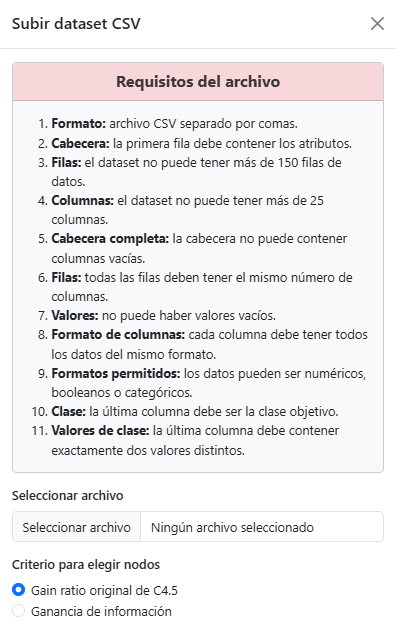
\includegraphics[width=0.5\textwidth]{img/Web_Arbol_C45_Subir_CSV.png}
     \caption{Ventana de subida de un dataset CSV}
     \label{Fig_E.11}
 \end{figure}

Los principales requisitos del archivo CSV son los siguientes:

\begin{itemize}
    \item el archivo debe estar separado por comas;
    \item la primera fila debe contener la cabecera con los nombres de los atributos;
    \item el dataset no puede superar las 150 filas de datos;
    \item el dataset no puede superar las 25 columnas;
    \item no puede haber columnas vacías en la cabecera;
    \item todas las filas deben tener el mismo número de columnas;
    \item no puede haber valores vacíos;
    \item los datos pueden ser numéricos, booleanos o categóricos;
    \item la última columna debe representar la clase objetivo;
    \item la clase objetivo debe contener exactamente dos valores distintos.
\end{itemize}

En la misma ventana se permite seleccionar el criterio utilizado para elegir los nodos del árbol. Por defecto se utiliza \textit{Gain Ratio}, que es el criterio propio del algoritmo C4.5. También se ofrece la posibilidad de utilizar ganancia de información como criterio alternativo con finalidad didáctica. Si se selecciona esta segunda opción, la aplicación muestra un aviso indicando que C4.5 original utiliza \textit{Gain Ratio}.

Una vez cargado un dataset válido, se activa la simulación paso a paso. La pantalla principal se divide en tres paneles:

\begin{itemize}
    \item \textbf{Árbol:} muestra la representación gráfica del árbol de decisión.
    \item \textbf{Dataset:} muestra la tabla de datos utilizada por el algoritmo.
    \item \textbf{Cálculos:} muestra las métricas calculadas en cada paso.
\end{itemize}

La figura \ref{Fig_E.12} muestra un ejemplo de los tres paneles de trabajo.

\begin{figure}[htbp]
     \centering
     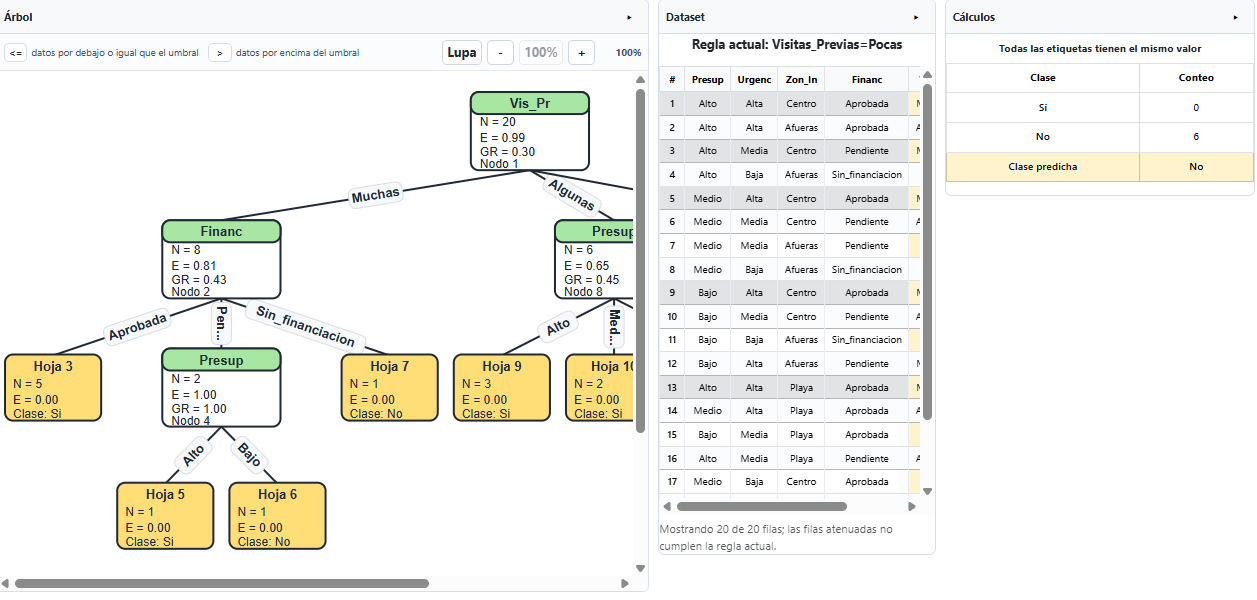
\includegraphics[width=1.2\textwidth]{img/Web_Arbol_C45_Paneles.png}
     \caption{Paneles de árbol, dataset y cálculos en la simulación C4.5}
     \label{Fig_E.12}
 \end{figure}

El panel del árbol representa visualmente los nodos y hojas generados. Cada nodo interno muestra información como el atributo seleccionado, el número de registros, la entropía y el valor de \textit{Gain Ratio}. Las hojas muestran la clase predicha y los valores asociados al subconjunto correspondiente.

Las ramas indican la condición que se aplica para pasar de un nodo a otro. En el caso de atributos numéricos, aparecen condiciones del tipo menor o igual que el umbral y mayor que el umbral. En el caso de atributos categóricos, la rama muestra el valor de la categoría correspondiente.

El panel del dataset muestra las filas del conjunto de datos. Durante la simulación, las filas que no cumplen las condiciones del paso actual aparecen atenuadas, de forma que el usuario puede identificar qué registros llegan al nodo que se está evaluando. Además, las columnas utilizadas en las condiciones activas se resaltan visualmente.

El panel de cálculos muestra la información utilizada para seleccionar cada nodo. En los nodos internos se presenta una tabla con las métricas calculadas para los atributos evaluados:

\begin{itemize}
    \item proporción de registros en cada división;
    \item número de registros de cada clase;
    \item entropía;
    \item entropía condicional;
    \item ganancia de información;
    \item \textit{Split Info};
    \item \textit{Gain Ratio}.
\end{itemize}

Cuando el paso actual corresponde a una hoja, el panel de cálculos muestra el conteo de registros de cada clase y la clase predicha por la hoja.

La navegación por la simulación se realiza mediante los botones situados sobre los paneles. Estos botones permiten:

\begin{itemize}
    \item ir al primer paso;
    \item retroceder al paso anterior;
    \item avanzar al paso siguiente;
    \item ir al último paso.
\end{itemize}

Al cambiar de paso, la aplicación actualiza de forma simultánea el árbol, el dataset y la tabla de cálculos. De esta manera, el usuario puede observar cómo se construye progresivamente el árbol y qué datos justifican cada decisión.

El panel del árbol incluye herramientas adicionales de visualización. El usuario puede aumentar o reducir el zoom del árbol, restaurar la escala al 100\% y activar una lupa para inspeccionar zonas concretas del SVG. También se muestra una pequeña leyenda para interpretar las ramas generadas por atributos numéricos.

Los paneles de árbol, dataset y cálculos son retráctiles. El usuario puede minimizar alguno de ellos para dar más espacio al resto, lo que resulta útil cuando se desea observar con más detalle el árbol o una tabla concreta.

En conjunto, la sección de simulación del árbol C4.5 permite al usuario realizar las siguientes acciones:

\begin{itemize}
    \item seleccionar un dataset de ejemplo;
    \item subir un dataset CSV propio;
    \item consultar los requisitos que debe cumplir el archivo CSV;
    \item elegir entre \textit{Gain Ratio} y ganancia de información como criterio de selección;
    \item visualizar el dataset cargado;
    \item construir el árbol de decisión paso a paso;
    \item observar qué registros llegan a cada nodo;
    \item consultar las métricas calculadas en cada división;
    \item visualizar nodos, hojas y ramas del árbol;
    \item ampliar, reducir o restaurar el zoom del árbol;
    \item utilizar la lupa para inspeccionar el árbol;
    \item contraer o expandir los paneles de trabajo;
    \item limpiar el dataset cargado y reiniciar la simulación.
\end{itemize}

\subsubsection{Poda del árbol}

La pestaña de poda permite al usuario estudiar cómo se simplifica el árbol generado. Esta sección parte del árbol completo construido con C4.5 y evalúa distintos subárboles para decidir si conviene mantenerlos o sustituirlos por una hoja.

La figura \ref{Fig_E.13} muestra la página de poda del árbol C4.5.

\begin{figure}[htbp]
     \centering
     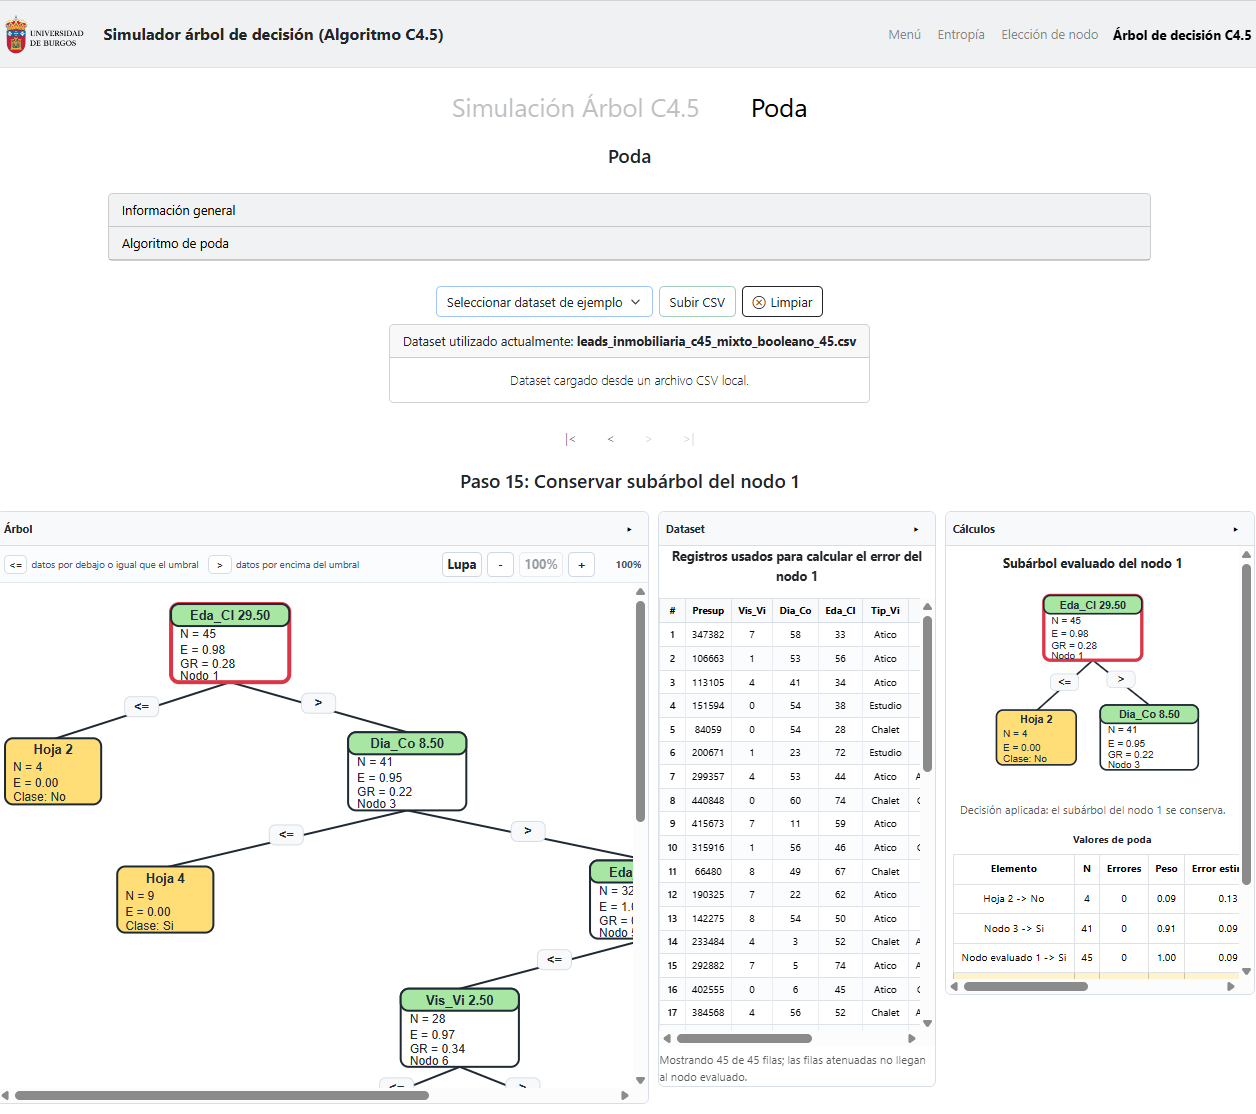
\includegraphics[width=1.2\textwidth]{img/Web_Arbol_C45_Poda.png}
     \caption{Visualización de la página de poda del árbol C4.5}
     \label{Fig_E.13}
 \end{figure}

La página de poda mantiene una estructura similar a la página de construcción del árbol. En la parte superior se muestran tarjetas informativas desplegables:

\begin{itemize}
    \item Tarjetas informativas en la parte superior.
    \begin{description}
        \item[Información general:] explica el objetivo de la poda y su utilidad para evitar árboles demasiado específicos.
        \item[Algoritmo de poda:] muestra cómo se compara el error estimado de un subárbol con el error de sustituirlo por una hoja.
    \end{description}
\end{itemize}

Al igual que en la simulación principal, el usuario puede seleccionar un dataset de ejemplo o subir un archivo CSV propio. Una vez cargado el dataset, la aplicación construye el árbol completo y genera los pasos del procedimiento de poda.

Durante la simulación de poda se utilizan los mismos tres paneles principales:

\begin{itemize}
    \item \textbf{Árbol:} muestra el estado del árbol en el paso actual de la poda.
    \item \textbf{Dataset:} resalta los registros que llegan al nodo o subárbol evaluado.
    \item \textbf{Cálculos:} muestra los errores estimados y la decisión tomada.
\end{itemize}

En cada paso se evalúa un subárbol candidato. La aplicación muestra el subárbol implicado, los registros que llegan al nodo evaluado y una tabla con los valores utilizados en la decisión. Esta tabla incluye información como:

\begin{itemize}
    \item número de registros que llegan a cada hoja;
    \item errores reales de cada hoja;
    \item peso de cada hoja dentro del subárbol;
    \item error estimado de cada hoja;
    \item error estimado total del subárbol;
    \item error estimado de la hoja simplificada;
    \item decisión final de podar o conservar.
\end{itemize}

Si el error estimado de sustituir el subárbol por una hoja es menor o igual que el error estimado del subárbol original, la aplicación muestra que el subárbol se poda. En caso contrario, se indica que el subárbol se conserva.

La navegación por la poda se realiza también mediante los botones de primer paso, paso anterior, paso siguiente y último paso. Al avanzar, el usuario puede observar cómo se evalúan los distintos subárboles y cómo cambia el árbol tras aplicar las decisiones de poda.

En conjunto, la sección de poda permite al usuario realizar las siguientes acciones:

\begin{itemize}
    \item cargar un dataset de ejemplo o un CSV propio;
    \item consultar la explicación teórica del procedimiento de poda;
    \item recorrer paso a paso la evaluación de subárboles;
    \item visualizar el subárbol evaluado en cada paso;
    \item observar los registros utilizados para calcular el error;
    \item comparar el error estimado del subárbol con el de una hoja simplificada;
    \item comprobar si el subárbol se poda o se conserva;
    \item visualizar el árbol resultante tras cada decisión;
    \item utilizar los mismos controles de zoom, lupa y paneles retráctiles que en la simulación principal.
\end{itemize}

Esta pestaña complementa la simulación de construcción del árbol, ya que permite observar no solo cómo se genera el modelo, sino también cómo puede simplificarse para evitar estructuras demasiado complejas.